\documentclass[12pt]{article}
\setlength{\oddsidemargin}{0in}
\setlength{\evensidemargin}{0in}
\setlength{\textwidth}{6.5in}
\setlength{\parindent}{0in}
\setlength{\parskip}{\baselineskip}

\usepackage{amsmath,amsfonts,amssymb,graphicx,xcolor}

%\title{Review of Newtonian Mechanics}

\newcommand{\purple}[1]{{\color{purple} #1}}

\begin{document}

PHYS 374 Fall 2020\hfill Worksheet 4: Revenge of the Frictionless Ramp\\
\\
Name: \purple{SOLUTION} \\
\\
Please submit as a PDF on Moodle. Include any calculations made using external tools.

\hrulefill
\\
\\
Let's revisit the mass on a frictionless ramp using calculus of variations. We are interested in the motion of the block down the ramp, as well as the motion of the ramp itself. 
\begin{figure}[h]
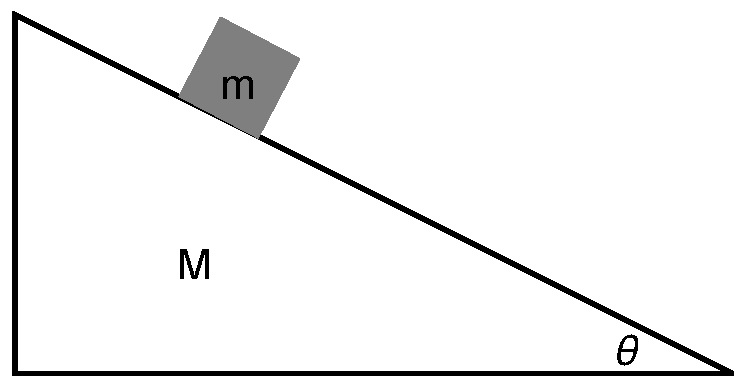
\includegraphics[width=5cm]{Diagram.pdf}
\centering
\end{figure}
\begin{enumerate}
\item Write down expressions for the position of the ramp and the position of the block. Make sure to use no more variables than the system has degrees of freedom.
\item What are the kinetic and potential energies associated with the ramp? Is there a more convenient reference point?
\item What are the kinetic and potential energies associated with the block? Is there a more convenient reference point?
\item Write down the Lagrangian of the system. Double check your signs!
\item Use the Euler-Lagrange equations to find the equations of motion.
\item Solve the equations to find the acceleration of the ramp and the acceleration of block along the surface of the ramp.
\item Does this system behave as expected when $M$ and/or $\theta$ take extreme values?
\item How does the Lagrangian solution compare to our earlier Newtonian solution for the same system?
\end{enumerate}

\purple{
Let's start out using rectangular coordinates. We can write the position of the ramp as $(X, Y)$ and the position of the block as $(x, y)$. Right away, we can ignore $Y$, since the ramp does not move vertically. But we're still using three variables ($x$, $y$, and $X$) to describe a system with only two degrees of freedom. 
\begin{figure}[h]
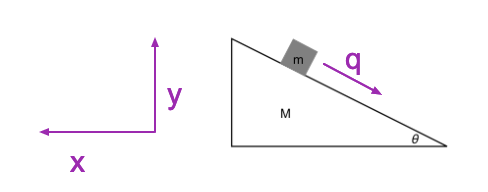
\includegraphics[width=10cm]{ramp-coords.png}
\centering
\end{figure}

We're happy using $X$ as one of our variables, since we care about the movement of the ramp. In order to conveniently talk about how far the block has moved, let's introduce a new variable: $q$, the distance the block has moved down the ramp. By looking at the horizontal and vertical displacement of the block (including the movement of the ramp) we see:
$$
x = q\cos\theta - X
\quad\quad \text{and} \quad\quad
y = -q\sin\theta
$$
As an aside, we could just as easily eliminate $x$ and $q$, leaving $X$ and $y$ as our two variables. The math works out pretty much the same either way, just with a few $\sin\theta$ and $\cos\theta$ moved around. 

To construct our Lagrangian, we need expressions for kinetic and potential energy. For the ramp, we start with:
$$
T_M = \tfrac{1}{2} M \left( \dot{X}^2 + \dot{Y}^2 \right)
\quad\quad \text{and} \quad\quad
U_M = MgY
$$
Note that $Y$ is a constant, so $\dot{Y}$ vanishes and we can measure our potential energy relative to the initial position rather than (say) relative to the table. Then:
$$
T_M = \tfrac{1}{2} M \dot{X}^2
\quad\quad \text{and} \quad\quad
U_M = 0
$$
Similarly, we can write out the kinetic and potential energy for the block in terms of our familiar coordinates $x$ and $y$:
$$
T_m = \tfrac{1}{2} m \left( \dot{x}^2 + \dot{y}^2 \right)
\quad\quad \text{and} \quad\quad
U_m = mgy
$$
Then rewrite those same expressions in terms of $q$ and $\dot{q}$:
$$
T_m = \tfrac{1}{2} m \left( \left( \dot{q} \cos\theta - \dot{X} \right)^2 + \left( -\dot{q} \sin\theta\right)^2 \right)
\quad\quad \text{and} \quad\quad
U_m = mgq\sin\theta
$$
The Lagrangian for this system is given by:
$$
\mathcal{L} = T_M + T_m - U_M - U_m
$$
Plugging in and expanding, that's:
$$
\mathcal{L} = \tfrac{1}{2} M \dot{X}^2 + \tfrac{1}{2} m \dot{X}^2 + \tfrac{1}{2} m \dot{q}^2 - m \dot{X} \dot{q} \cos\theta + m g q \sin\theta
$$
Our variables are $X$ and $q$ so our Euler-Lagrange equations are:
$$
\frac{\partial\mathcal{L}}{\partial X} = \frac{d}{dt} \left( \frac{\partial\mathcal{L}}{\partial \dot{X}} \right)
\quad\quad \text{and} \quad\quad
\frac{\partial\mathcal{L}}{\partial q} = \frac{d}{dt} \left( \frac{\partial\mathcal{L}}{\partial \dot{q}} \right)
$$
Let's tackle $X$ first. Evaluating our derivatives:
$$
\frac{\partial\mathcal{L}}{\partial X} = 0
\quad\quad \text{and} \quad\quad
\frac{\partial\mathcal{L}}{\partial \dot{X}} = M\dot{X} + m\dot{X} - m\dot{q}\cos\theta
$$
So:
$$
0 = \frac{d}{dt} \left( M\dot{X} + m\dot{X} - m\dot{q}\cos\theta \right)
\quad\quad \text{or} \quad\quad
M\dot{X} + m\dot{X} - m\dot{q}\cos\theta = p
$$
Where $p$ is a constant. Specifically, $p$ is the horizontal momentum of the system, which is conserved. The terms $M\dot{X} + m\dot{X}$ reflect the momentum of the ramp to the left, carrying the block with it, and $m\dot{q}\cos\theta$ is the horizontal component of the block's momentum to the right. The system started at rest, so we can say $p=0$, or:
$$
M\dot{X} + m\dot{X} = m\dot{q}\cos\theta
\quad\rightarrow\quad
\dot{X} = \dot{q} \tfrac{m}{M+m} \cos\theta
$$
Now let's look at the Euler-Lagrange equation for $q$:
$$
\frac{\partial\mathcal{L}}{\partial q} = mg\sin\theta
\quad\quad \text{and} \quad\quad
\frac{d}{dt} \left( \frac{\partial\mathcal{L}}{\partial \dot{q}} \right) = m\ddot{q} - m\ddot{X}\cos\theta
$$
Or:
$$
mg\sin\theta = m\ddot{q} - m\ddot{X}\cos\theta
$$
We can recognize this equation too. On the left, $mg\sin\theta$ is the component of the net force on the block perpendicular to the ramp surface. On the right is the acceleration of the block in that same direction. One term for movement down the ramp, another term for that component of the movement of the block carried by the ramp.

With a bit of rearranging, we can solve to get:
$$
\ddot{q} = \frac{g\sin\theta}{1 - \tfrac{m}{M+m} \cos^2\theta}
\quad \quad \text{and} \quad \quad
\ddot{X} = \frac{g \sin\theta \cos\theta}{ \tfrac{M + m}{m} - \cos^2\theta}
$$
Above, $\ddot{X}$ is the acceleration of the ramp to the left, and $\ddot{q}$ is the acceleration of the block down the ramp. We can take a look at a few limiting cases:
\begin{itemize}
    \item If $\theta \rightarrow 0$ then nothing moves
    \item If $\theta \rightarrow \tfrac{\pi}{2}$ then the ramp stays still and the block accelerates (straight down) at $g$
    \item If $M\rightarrow \infty$ then the block accelerates down the ramp at $g\sin\theta$ and the ramp does not move
    \item If $M \rightarrow 0$ then the block accelerates down the ramp at $\frac{g}{\sin\theta}$ while the ramp accelerates out of the way at $g\cot\theta$. In this case, it's helpful to draw out horizontal and vertical components to understand what's going on. The vertical component of $\ddot{q}$ is $g$, while the horizontal components of $\ddot{X}$ and $\ddot{q}$ are equal and opposite. In effect, the block falls straight down at $g$, shoving the ramp out of the way as it goes. 
\end{itemize}
Your experience is your own! 

In my opinion, this problem is difficult to get started using the Newtonian formulation. It's not obvious how to choose coordinates. The normal force looks like it might be constant, but isn't. There are a ton of dead ends before you write down anything that matters.

The Lagrangian process is more math, but also more straightforward. Write down the energies, crunch out some derivatives, and you're good to go. The results are most intuitive when solved using $X$ and $q$, but we could have gotten the same answer using $X$ and $y$, or even $X$ and $x$! 

}
\end{document}